\documentclass[conference]{IEEEtran}
\IEEEoverridecommandlockouts
\usepackage{amsmath,amssymb,amsfonts}
\usepackage{graphicx}
\usepackage{array}
\usepackage{url}
\usepackage[T1]{fontenc}
\usepackage{textcomp}
\begin{document}
\title{IntelliBot: Autonomous Mobile Manipulator for Warehouse Pick-and-Place\\[4pt] {\normalsize Code: \texttt{https://github.com/Multi-meta/RI-Project}}}
\author{\IEEEauthorblockN{Abhishek Anand}\IEEEauthorblockA{\textit{Robotic Intelligence, course project}}
\and
\IEEEauthorblockN{Ankit Kumar}\IEEEauthorblockA{\textit{Robotic Intelligence, course project}}
\and
\IEEEauthorblockN{Utkarsh Yuvraj}\IEEEauthorblockA{\textit{Robotic Intelligence, course project}}}
\maketitle
\begin{abstract}
IntelliBot completes a full pick-and-place mission in simulation: it finds parcel P3 with its cameras, picks it with a 3-joint arm, carries it past moving traffic and places it on the Zone B rack in 72.9 s, 0.6 cm from the slot centre, with zero contacts. We built a miniature warehouse in the Webots simulator and a differential-drive mobile manipulator for it, carrying a 360-ray LiDAR, front and rear cameras, GPS, an IMU, wheel encoders and two bumpers. Everything runs in a closed loop in Python: a colour detector finds the parcel, A* plans a route on an inflated occupancy grid, a PID waypoint follower drives it, and a finite-state machine sequences the mission. Three features make the robot robust rather than scripted: an Extended Kalman Filter (EKF) fuses odometry, GPS and IMU, gates out bad readings and falls back to dead reckoning when GPS is lost; a dynamic obstacle layer built from LiDAR triggers replanning from the current pose; and a speed governor limits velocity to what the robot can stop within, given the measured clearance. In Webots the EKF tracks ground truth with 5 mm position and 0.12$^\circ$ heading RMSE, and a Webots memory leak that crashed long runs was found and fixed.
\end{abstract}
\begin{IEEEkeywords}
mobile manipulation, extended Kalman filter, sensor fusion, A* path planning, warehouse automation, Webots
\end{IEEEkeywords}

\section{Introduction}
Warehouse robots must find goods, move them through shared aisles and put them away without a human steering them. This project builds that capability end to end, in simulation, at a scale a student team can explain line by line.

\subsection{Motivation}
Autonomous mobile robots now move a large share of goods in fulfilment centres. The hard part is not driving a known route but staying correct when the world disagrees with the plan: a parcel is not exactly where expected, a cart blocks the aisle, or a sensor drops out. A robot that only replays a recorded path fails at the first surprise. We wanted a robot whose every action comes from what it senses in the moment.

\subsection{Problem Statement}
Given the task ``pick package P3 and deliver it to Zone B'', the robot must:

\begin{enumerate}
\item find the parcel with its own sensors, not from a map entry;
\item plan a collision-free route on a known warehouse map;
\item drive the route while avoiding static and moving obstacles;
\item dock precisely enough for an arm to grasp a 20 cm parcel;
\item carry it to the destination rack and place it in a free slot;
\item verify the result and write a mission report.
\end{enumerate}
A hard-coded route or a teleported parcel is explicitly not acceptable: the parcel must be held by the gripper and moved by physics.

\subsection{Objectives}
\begin{itemize}
\item Model a warehouse world and a mobile manipulator in Webots~\cite{r1}, generated from one configuration file so the map and the world can never disagree.
\item Implement differential-drive kinematics, odometry and PID heading control~\cite{r4},~\cite{r10}, and validate them against ground truth.
\item Detect parcels by colour with OpenCV~\cite{r8} and estimate their position from camera bearing plus LiDAR range.
\item Plan with A*~\cite{r3} on an inflated occupancy grid and replan from the current pose when the route is blocked.
\item Fuse odometry, GPS and IMU with an EKF~\cite{r2} that rejects outliers and degrades gracefully.
\item Bound speed by stopping distance so the robot never outruns its sensors.
\item Pick and place with a 3-joint arm~\cite{r5} and a latching gripper, with sensor-based verification.
\item Test robustness with moving obstacles, and report measured numbers only.
\end{itemize}
\subsection{Scope}
The work is simulation only. Localisation uses GPS, IMU and wheel odometry; there is no SLAM. One robot works at a time; the multi-robot world exists but was not evaluated. All results are from Webots runs or from an offline kinematic simulator, and each number says which.

\subsection{Paper Outline}
Section II describes the world, the robot and the software. Section III presents measured results with graphs and simulator screenshots, and discusses the problems we found. Sections IV and V conclude and list future work.

\section{Methodology: Working Model, Simulation and Code}
The robot runs a sense--decide--act loop every 16 ms: sensors feed perception and the EKF, a state machine picks the next action, a planner and controller turn it into wheel and arm commands, and every step is logged.

\subsection{Simulation World}
The warehouse is an 8 m $\times$ 6 m walled floor in Webots R2025a (16 ms physics step, ENU frame). \texttt{tools/generate\_\allowbreak{}world.py} writes the world file from \texttt{config.py}, so the occupancy grid the robot plans on and the world it drives in come from the same numbers. A supervisor check compares object positions with the configuration at start-up and warns on any mismatch over 1 cm. Table I lists the world elements and Fig. 1 shows the generated world.

\begin{table*}[!t]
\caption{Simulation world elements}
\centering
\footnotesize
\renewcommand{\arraystretch}{1.2}
\begin{tabular}{p{0.2\linewidth}p{0.45\linewidth}p{0.27\linewidth}}
\hline
\textbf{Element} & \textbf{Position / size} & \textbf{Purpose} \\ \hline
4 shelves & 1.6 $\times$ 0.5 $\times$ 1.0 m at ($\pm$2.0, $\pm$1.9) & static aisles \\
Crates, barrels, ball & 0.3--0.4 m boxes; $r$ = 0.12--0.15 m cylinders; $r$ = 0.15 m sphere & varied obstacle shapes \\
Pickup area & 1.2 $\times$ 1.6 m at ($-$3.0, 0.0) & parcels P1 (red), P2 (green), P3 (blue): 0.2 m cubes, 0.5 kg \\
Zone A / Zone B & 1 $\times$ 1 m patches at (3.0, $\pm$0.9), yellow / cyan & dispatch zones \\
Destination racks A / B & east wall; levels at 0.15, 0.41, 0.67 m & placement slots (L1, L2 reachable) \\
CART\_1, CART\_2 & patrol $y$ = 2.4 at 0.4 m/s; cross aisle $x$ = 0.72 at 0.3 m/s & moving traffic \\
DECOY\_BOT & yellow look-alike robot, $x = -1.5$, $y \in [-1.20, 0.15]$, 0.25 m/s & crosses the start-to-pickup route and gives way \\
\hline
\end{tabular}
\end{table*}
\begin{figure}[!t]
\centering
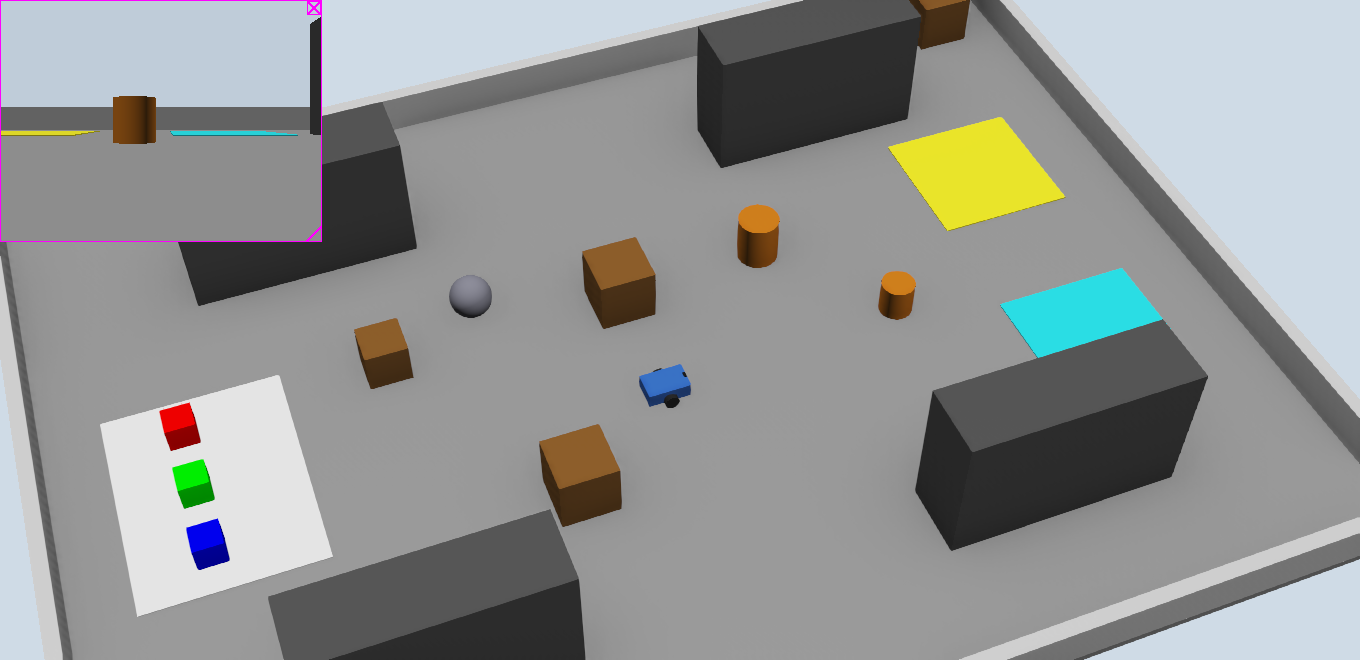
\includegraphics[width=\columnwidth]{figures/fig1_world.png}
\caption{The generated warehouse in Webots: pickup area with parcels P1--P3 (left), shelves, varied obstacles, Zone A (yellow) and Zone B (cyan) with destination racks (right), and IntelliBot (blue). Inset: the robot's front camera.}
\end{figure}
\subsection{Robot Model}
IntelliBot is a differential-drive base (0.30 $\times$ 0.20 $\times$ 0.10 m, 2.8 kg) with two driven wheels ($r$ = 0.05 m, track $L$ = 0.24 m, 20 rad/s limit) and two zero-friction casters. A post at the rear carries the arm. Table II lists its devices.

\begin{table*}[!t]
\caption{Robot devices}
\centering
\footnotesize
\renewcommand{\arraystretch}{1.2}
\begin{tabular}{p{0.2\linewidth}p{0.45\linewidth}p{0.27\linewidth}}
\hline
\textbf{Device} & \textbf{Specification} & \textbf{Used for} \\ \hline
LiDAR & 360 rays, 360$^\circ$, 0.05--4.0 m, 0.14 m high & obstacles, docking, dynamic map \\
Front and rear cameras & 320 $\times$ 240, 1.0 rad planar FOV, 0.12 m high & parcel detection, camera health \\
GPS + IMU & position $(x, y)$ and yaw & EKF corrections \\
Wheel encoders & position sensors on both wheels & odometry (EKF prediction) \\
Front and rear bumpers & touch sensors & collision events and recovery \\
Arm & shoulder, elbow, wrist pitch joints; links 0.28 m and 0.25 m & pick from floor, place on rack \\
Gripper & two fingers, 0.12 m travel each, force pads, palm range sensor, Connector latch & grasp, verify, hold the parcel \\
Display, LED, pen & 320 $\times$ 240 dashboard, state colour, floor trail & live monitoring and evidence \\
\hline
\end{tabular}
\end{table*}
\subsection{Software Architecture}
The controller (\texttt{intellibot\_\allowbreak{}controller.py}) is a Webots supervisor written in Python 3.12 with NumPy~\cite{r9} and OpenCV~\cite{r8}. Only it and \texttt{perception.py} touch the Webots API; every algorithm (kinematics, PID, grid, A*, EKF, FSM, detector, docking, arm kinematics) is plain Python, so it can be unit-tested without the simulator. All constants live in \texttt{config.py}. Fig. 2 shows the data flow. The FSM is the only place that decides; perception and the EKF only report, and the governor can always overrule a speed command.

\begin{figure}[!t]
\centering
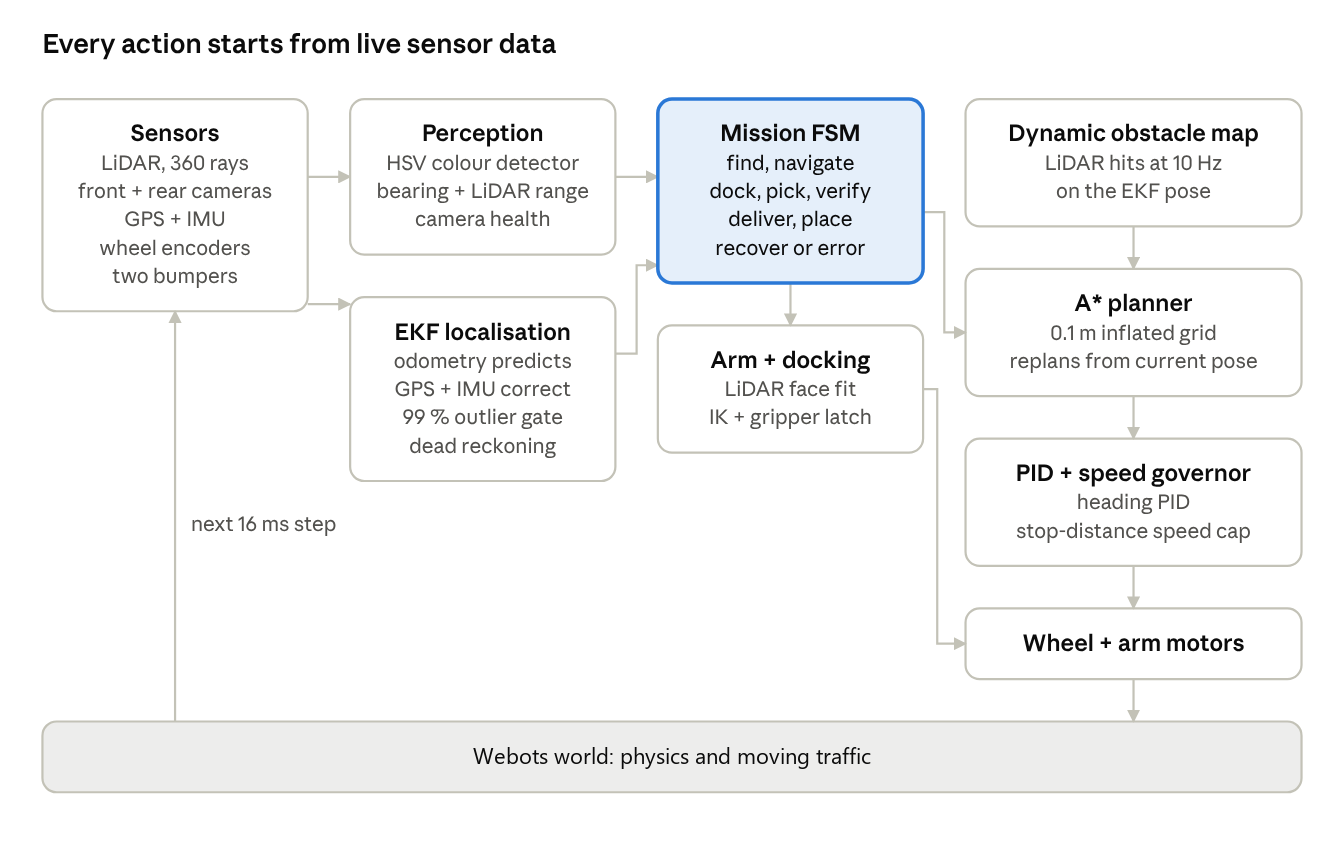
\includegraphics[width=\columnwidth]{figures/fig2_architecture.png}
\caption{Control architecture: data flow in one 16 ms control step.}
\end{figure}
\subsection{Kinematics and Motion Control}
A body command $(v, \omega)$ maps to wheel speeds by inverse kinematics~\cite{r4}:

\begin{equation}
\omega_L = \frac{v - \omega L/2}{r}, \qquad \omega_R = \frac{v + \omega L/2}{r}
\label{eq:ik}
\end{equation}
and the encoder increments $\Delta\phi_L, \Delta\phi_R$ give the odometry update

\begin{equation}
\Delta s = \frac{r\,(\Delta\phi_R + \Delta\phi_L)}{2}, \qquad \Delta\theta = \frac{r\,(\Delta\phi_R - \Delta\phi_L)}{L}
\label{eq:odom}
\end{equation}
The waypoint follower steers with a PID on heading error, with gains $k_p = 2.0$, $k_i = 0.05$ and $k_d = 0.15$~\cite{r10}, turns in place when the error exceeds 0.6 rad, and slows over the last 0.5 m. It can drive forwards or backwards, whichever needs the smaller turn, because the robot has a camera at each end.

\subsection{Perception}
\begin{itemize}
\item \textbf{Parcel detection.} Each camera frame goes BGR to HSV; masks for red, green and blue are cleaned with morphology, then blobs are filtered by area and aspect ratio. The hue windows avoid the yellow and cyan zone colours and the yellow decoy robot. A detection must persist for 2 frames.
\item \textbf{Parcel position.} The pixel column gives a bearing; the LiDAR range in a $\pm 3^\circ$ window around that bearing gives the distance. The arm post blinds $\pm 6^\circ$ behind the LiDAR, so the robot first turns a rear-sector parcel out of that blind zone.
\item \textbf{LiDAR.} Ray order and offset were measured in Webots (index increases clockwise, $+0.02$ rad offset). Returns closer than 0.15 m are the robot itself and are discarded.
\item \textbf{Camera health.} Each frame is checked for BLANK and FROZEN (30 identical frames while moving) images. An unhealthy camera is ignored instead of trusted.
\end{itemize}
\begin{figure}[!t]
\centering
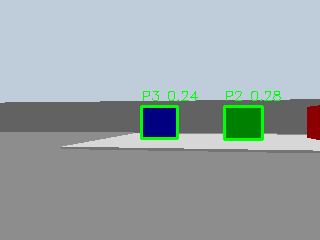
\includegraphics[width=\columnwidth]{figures/fig3_detector.png}
\caption{Detector output on a 320 $\times$ 240 front-camera frame from Webots: P3 (blue) and P2 (green) boxed with their confidence; the red parcel at the edge is partly out of view.}
\end{figure}
\begin{figure}[!t]
\centering
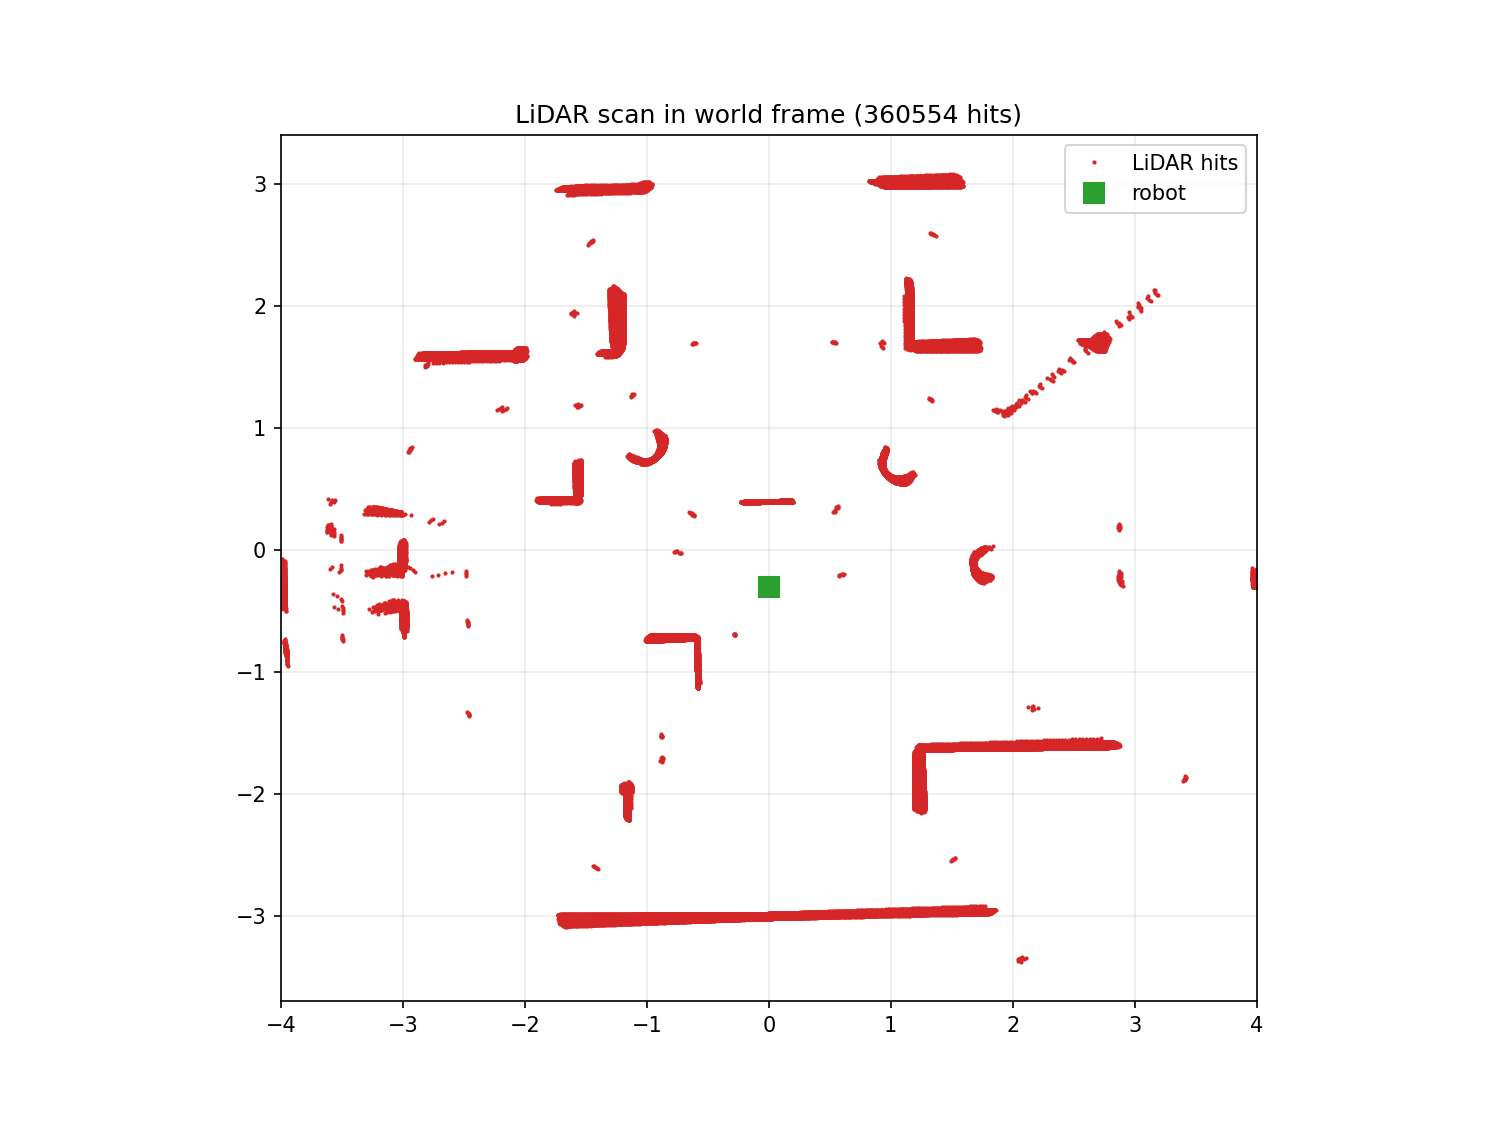
\includegraphics[width=\columnwidth]{figures/fig4_lidar.png}
\caption{LiDAR hits from a Webots run transformed into the world frame with the measured ray order and offset (360,554 points). Shelf edges, crates and walls line up with the map, which validated the calibration.}
\end{figure}
\subsection{Localisation: Extended Kalman Filter}
The state is the pose $\mathbf{x} = [x, y, \theta]^{\mathsf T}$. Odometry drives the prediction~\cite{r2}:

\begin{equation}
\hat{\mathbf{x}}_{k|k-1} = \hat{\mathbf{x}}_{k-1} + \begin{bmatrix} \Delta s\cos\theta_{k-1} \\ \Delta s\sin\theta_{k-1} \\ \Delta\theta \end{bmatrix}
\label{eq:pred}
\end{equation}
\begin{equation}
P_{k|k-1} = F_k P_{k-1} F_k^{\mathsf T} + Q_k(\Delta s, \Delta\theta)
\label{eq:cov}
\end{equation}
and GPS and IMU correct it with innovation $\boldsymbol{\nu}_k = \mathbf{z}_k - H\hat{\mathbf{x}}_{k|k-1}$ and gain

\begin{equation}
S_k = H P_{k|k-1} H^{\mathsf T} + R, \qquad K_k = P_{k|k-1} H^{\mathsf T} S_k^{-1}
\label{eq:gain}
\end{equation}
Every correction is gated by its normalised innovation squared, $\boldsymbol{\nu}_k^{\mathsf T} S_k^{-1} \boldsymbol{\nu}_k < \gamma$, with $\gamma = 9.21$ for GPS and 6.63 for the IMU ($\chi^2$, 99 \%)~\cite{r7}. A sensor's $R$ is inflated as its health drops. If GPS is silent for 0.5 s the filter dead-reckons on odometry and IMU. If GPS fixes are rejected but agree with each other for 0.5 s, the robot was displaced (for example by a collision), so it relocalises and the planner is told. A matching re-anchor exists for the IMU heading. The navigation pose is the EKF output; ground truth is read only for evaluation.

\subsection{Mapping, Planning and Replanning}
The static map is a 0.1 m occupancy grid inflated by the robot radius plus a 7 cm margin (0.25 m). A*~\cite{r3} (8-connected, Euclidean heuristic) finds a path, which is smoothed by line-of-sight shortcuts and resampled every 0.3 m. A dynamic layer marks cells from LiDAR hits at 10 Hz and clears them when rays pass through, so a moved obstacle disappears within four scans. The decision maker replans from the current pose when the next 1.5 m of route is blocked, the robot deviates more than 0.6 m, it is stuck for 5 s, it bumps something or the EKF relocalises. For a moving obstacle it first waits up to 4 s before detouring.

\subsection{Speed Governor}
Every command passes a governor that caps speed so the robot can always stop before the nearest obstacle in its corridor:

\begin{equation}
v_{\mathrm{cap}} = \min\left(v_{\mathrm{cruise}},\, v_{\mathrm{clear}},\, v_{\mathrm{carry}},\, v_{\mathrm{approach}},\, v_{\mathrm{health}}\right)
\label{eq:vcap}
\end{equation}
where $v_{\mathrm{clear}}$ is the largest speed whose stopping distance fits the measured clearance,

\begin{equation}
d_{\mathrm{stop}}(v) = v\, t_{\mathrm{react}} + \frac{v^{2}}{2\, a_{\mathrm{brake}}} + d_{\mathrm{margin}}
\label{eq:dstop}
\end{equation}
Cruise is 0.70 m/s, 0.50 m/s while carrying, 0.12 m/s with degraded LiDAR or localisation, and zero if the LiDAR fails. Acceleration is limited to 1.0 m/s$^2$ and yaw acceleration to 9 rad/s$^2$; an emergency stop skips the ramp.

\subsection{Mission State Machine}
The decision maker is a finite-state machine (Fig. 5): ARM\_STOW, FIND\_PACKAGE, NAVIGATE, DOCK\_PICK, ARM\_PICK, VERIFY\_ATTACHMENT, PLAN\_DELIVERY, DELIVER, DOCK\_PLACE, ARM\_PLACE, VERIFY\_DELIVERY and DONE, with ARM\_RECOVER and ERROR for failures. Each state has a timeout and logs its reason on exit. In interactive mode the robot asks for the next task at the console and returns to the centre between missions. Every step ends on a sensor check: the grasp is verified by finger width and force pads, the placement by the palm range-finder. Rack docking and placing retry in the same way.

\begin{figure*}[!t]
\centering
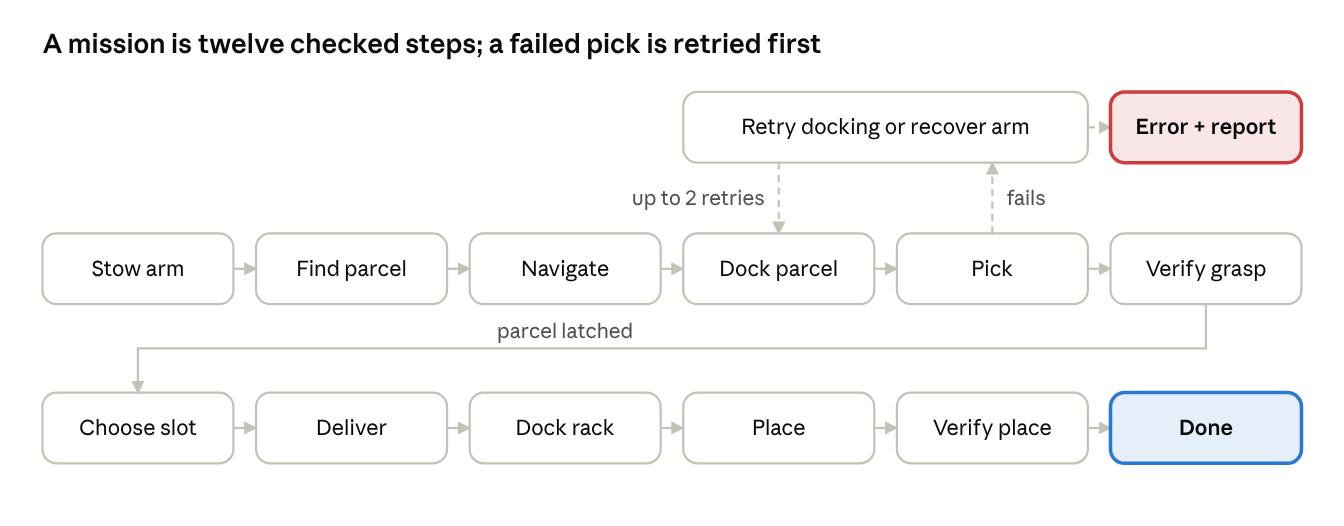
\includegraphics[width=0.9\textwidth]{figures/fig5_fsm.png}
\caption{Mission state machine (\texttt{decision\_\allowbreak{}maker.py}).}
\end{figure*}
\subsection{Manipulation and Docking}
Docking fits a line to the parcel's or rack's front face in the LiDAR scan, drives to a pre-dock point 0.20 m back on that line, then creeps in until range, lateral and heading errors are under 8 mm, 15 mm and 1.5$^\circ$. The arm then follows joint trajectories from planar inverse kinematics~\cite{r5}: pre-grasp, grasp at floor level, close the fingers, and lock the Connector latch. A grasp is accepted only if the finger width and force pads agree with a 20 cm parcel. At the rack the robot picks a free slot (levels L1 or L2), docks, places, releases and verifies that the parcel stayed in the slot (Fig. 6).

\begin{figure*}[!t]
\centering
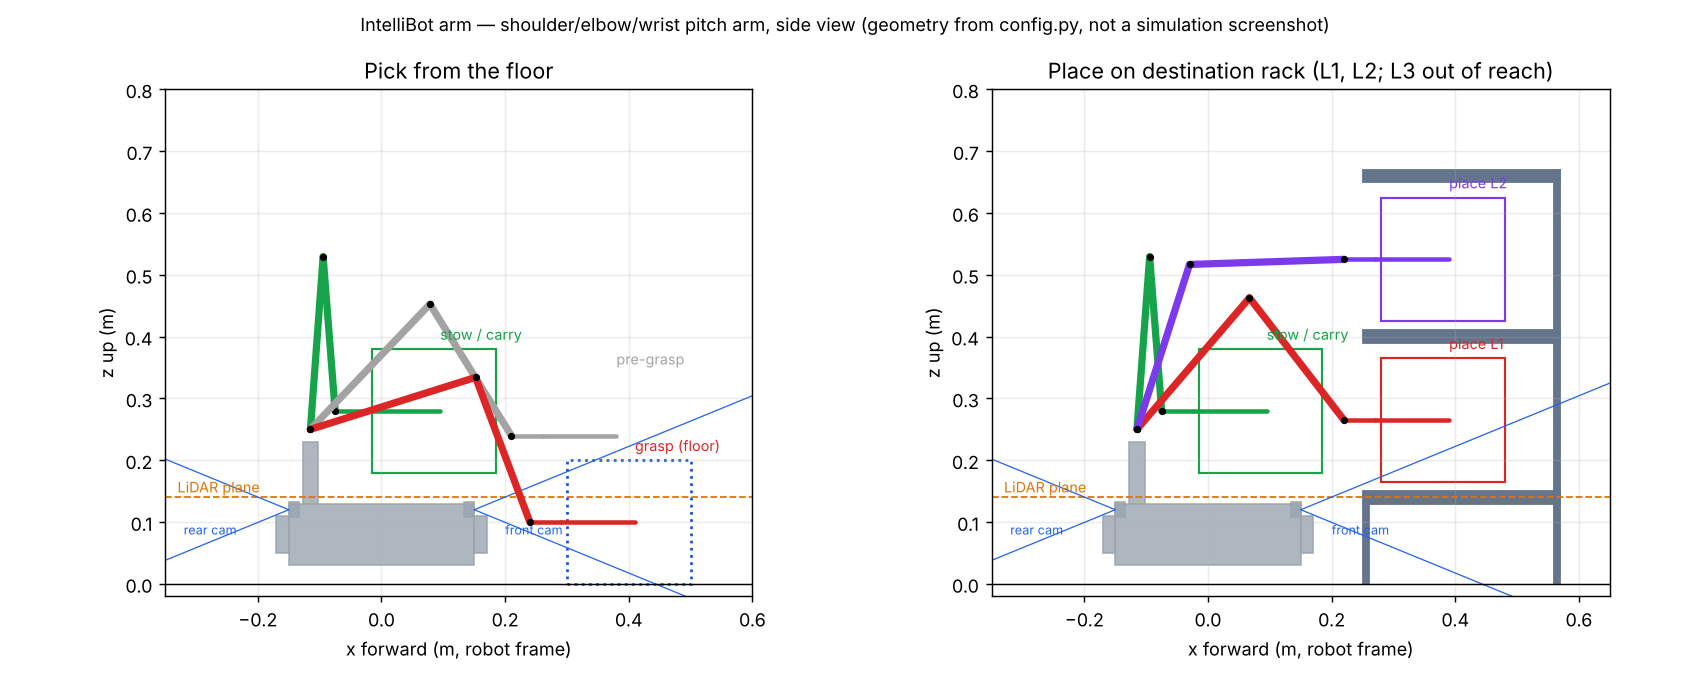
\includegraphics[width=0.9\textwidth]{figures/fig6_arm.png}
\caption{Arm geometry from \texttt{config.py} (side view, robot frame): stow/carry pose, pre-grasp and floor grasp (left); placing on rack levels L1 and L2 (right). Level 3 is out of reach. The orange line is the LiDAR plane the arm must stay clear of while stowed.}
\end{figure*}
\subsection{Moving Obstacles}
The carts and the decoy robot are moved kinematically by the supervisor, which writes their pose each step. An earlier design forced their velocity on physics bodies, which shoved the robot with unlimited force and sometimes froze them when the physics engine put the body to sleep. Each mover now runs its own small state machine (DRIVE, TURN, YIELD, BACKOFF, HOLD): it stops when IntelliBot is ahead within 0.45 m, backs up 0.45 m if the robot has not passed after 4 s, then carries on. The decoy turns round at each lane end, spins its wheels and flashes its beacon while giving way. IntelliBot is told none of this; it sees an obstacle on its sensors.

\subsection{Code Organisation and Testing}
The controller package has about 40 modules. 312 pytest tests cover kinematics, PID, grid, A*, EKF, safety, detector, docking, arm kinematics, the FSM, the movers and world generation, and run without Webots in about 90 s. An offline kinematic simulator runs whole missions for ablation studies. In Webots, each run writes \texttt{run.csv} (10 Hz state, poses, ground truth, speed caps), \texttt{manip.csv} (arm and gripper), \texttt{mission\_\allowbreak{}report.json} and a console log. Scenarios (normal runs and ablations) run in batch with \texttt{tools/run\_\allowbreak{}scenario.py}.

\section{Results and Discussion}
The full mission works in Webots: P3 is found, picked, carried and placed on the Zone B rack in 72.9 s, 0.6 cm from the slot centre, with no contacts and 5 mm localisation error. Every number below states whether it comes from Webots or from the offline kinematic simulator.

\subsection{Full Mission in Webots}
\begin{table}[!t]
\caption{Full mission in Webots (P3 to Zone B, batch run)}
\centering
\footnotesize
\renewcommand{\arraystretch}{1.2}
\begin{tabular}{p{0.42\linewidth}p{0.48\linewidth}}
\hline
\textbf{Measure} & \textbf{Value} \\ \hline
Result & DELIVERED, verified by sensors and by ground-truth audit \\
Mission time & 72.9 s simulated \\
Placement error & 0.6 cm from slot centre \\
Bumper contacts & 0 \\
EKF error vs ground truth & 5 mm position RMSE, 0.12$^\circ$ heading RMSE \\
Mean NEES & 0.37 (consistent: below 3 for a 3-state pose) \\
Cruise speed & 0.70 m/s (0.50 m/s carrying) \\
\hline
\end{tabular}
\end{table}
An interactive GUI run on the final build (decoy robot on the lane) delivered P1 to Zone A rack slot RA-L1-B1 in 93.6 s, with 17.5 m driven and one PATH\_BLOCKED replan. The EKF tracked ground truth with 5.7 mm and 0.17$^\circ$ RMSE (mean NEES 0.49, 1183 samples). There were no bumper contacts and no emergency stops; minimum corridor clearance was 0.07 m. The decoy robot gave way twice; CART\_2 gave way twice and backed up both times (Figs. 7 and 8).

\begin{figure}[!t]
\centering
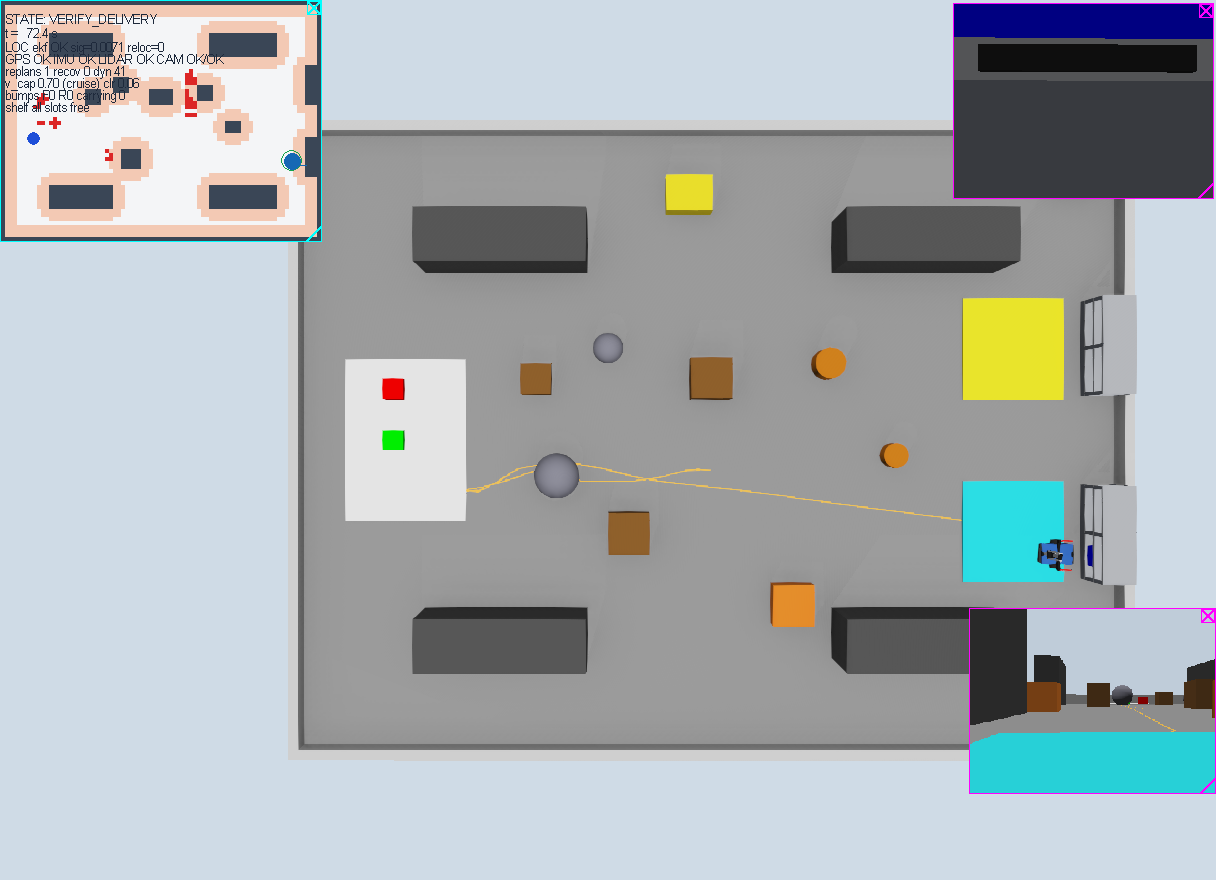
\includegraphics[width=\columnwidth]{figures/fig7_delivery.png}
\caption{Webots, end of a P3-to-Zone-B delivery at $t$ = 72.4 s (top view). The yellow trail is the path driven. Top left: the on-robot dashboard (state VERIFY\_DELIVERY, EKF $\sigma$ 7 mm, all sensors OK, cruise cap 0.70 m/s, no bumps). Right: front and rear camera views.}
\end{figure}
\begin{figure*}[!t]
\centering
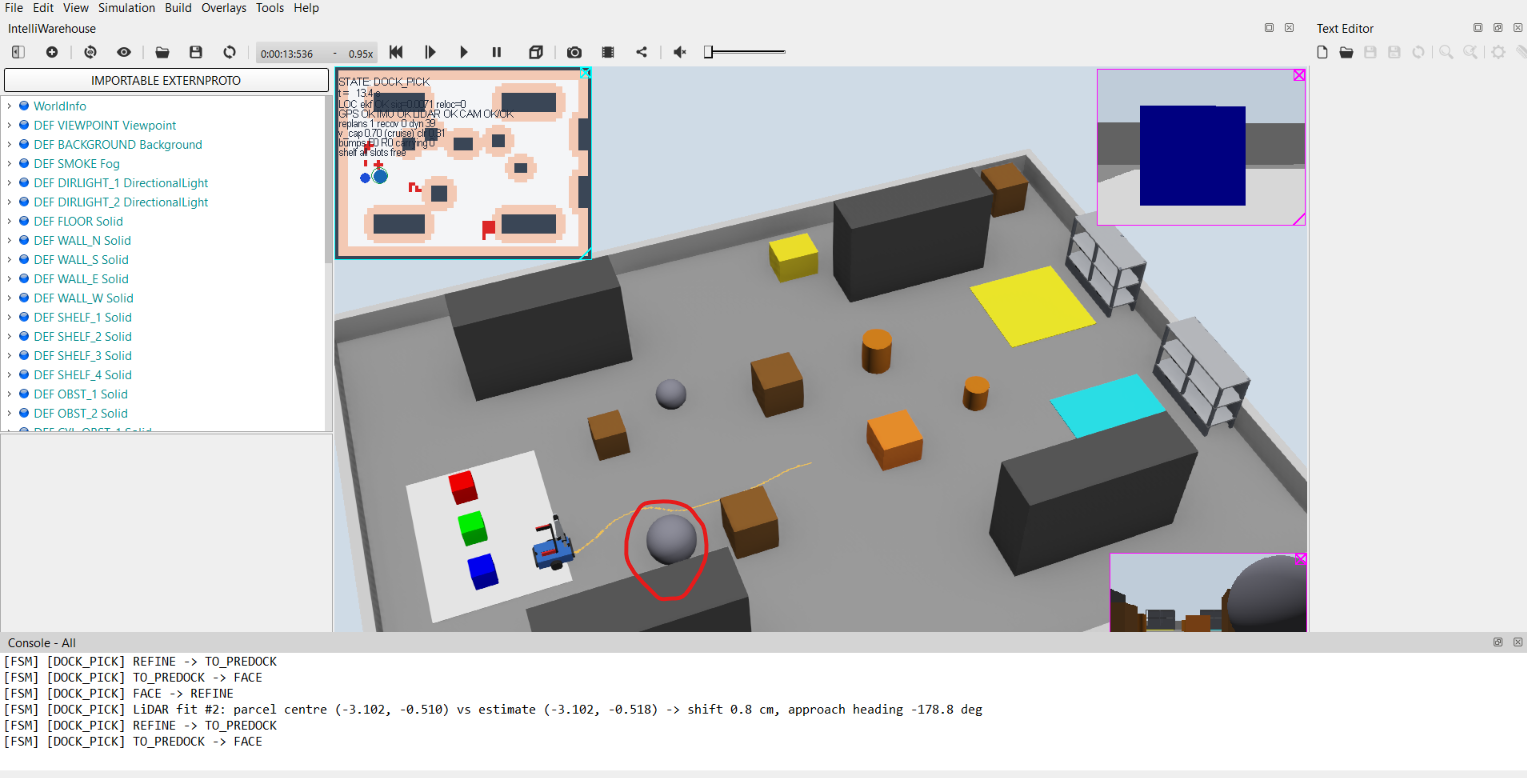
\includegraphics[width=0.9\textwidth]{figures/fig8_ui.png}
\caption{The Webots user interface during a mission (state DOCK\_PICK, $t$ = 13.4 s): scene tree with its nodes (left), dashboard and camera overlays, and the console log of the LiDAR docking fit (bottom). Captured before the grey sphere obstacle was replaced by the yellow decoy robot.}
\end{figure*}
\subsection{Kinematics and Odometry}
Commanded and measured motion agree within 1 \% (Table IV), which validates the wheel model before anything is built on it.

\begin{table}[!t]
\caption{Commanded vs measured motion in Webots}
\centering
\footnotesize
\renewcommand{\arraystretch}{1.2}
\begin{tabular}{ccccc}
\hline
\textbf{$v_{\mathrm{cmd}}$ (m/s)} & \textbf{$\omega_{\mathrm{cmd}}$ (rad/s)} & \textbf{$v$ meas.} & \textbf{$\omega$ meas.} & \textbf{Error} \\ \hline
0.20 & 0.00 & 0.1982 & 0.0000 & $-$0.90 \% \\
0.00 & 1.00 & 0.0000 & 0.9906 & $-$0.94 \% \\
0.20 & 0.50 & 0.1982 & 0.4953 & $-$0.90 \%, $-$0.94 \% \\
$-$0.10 & 0.00 & $-$0.0991 & 0.0000 & +0.90 \% \\
\hline
\end{tabular}
\end{table}
Pure odometry drifts 0.8--2.2 cm over 1--2 m and up to 4.7$^\circ$ after a square path. That is small per metre but unbounded over a mission, which is why odometry only drives the EKF's prediction.

\subsection{Path Tracking}
On an early full mission run, the robot followed the A* reference with a mean cross-track error of 0.4 cm and a maximum of 6.2 cm (723 samples, 69 s). The largest errors occur at the turn into the pickup area, where the follower turns in place (Fig. 9).

\begin{figure}[!t]
\centering
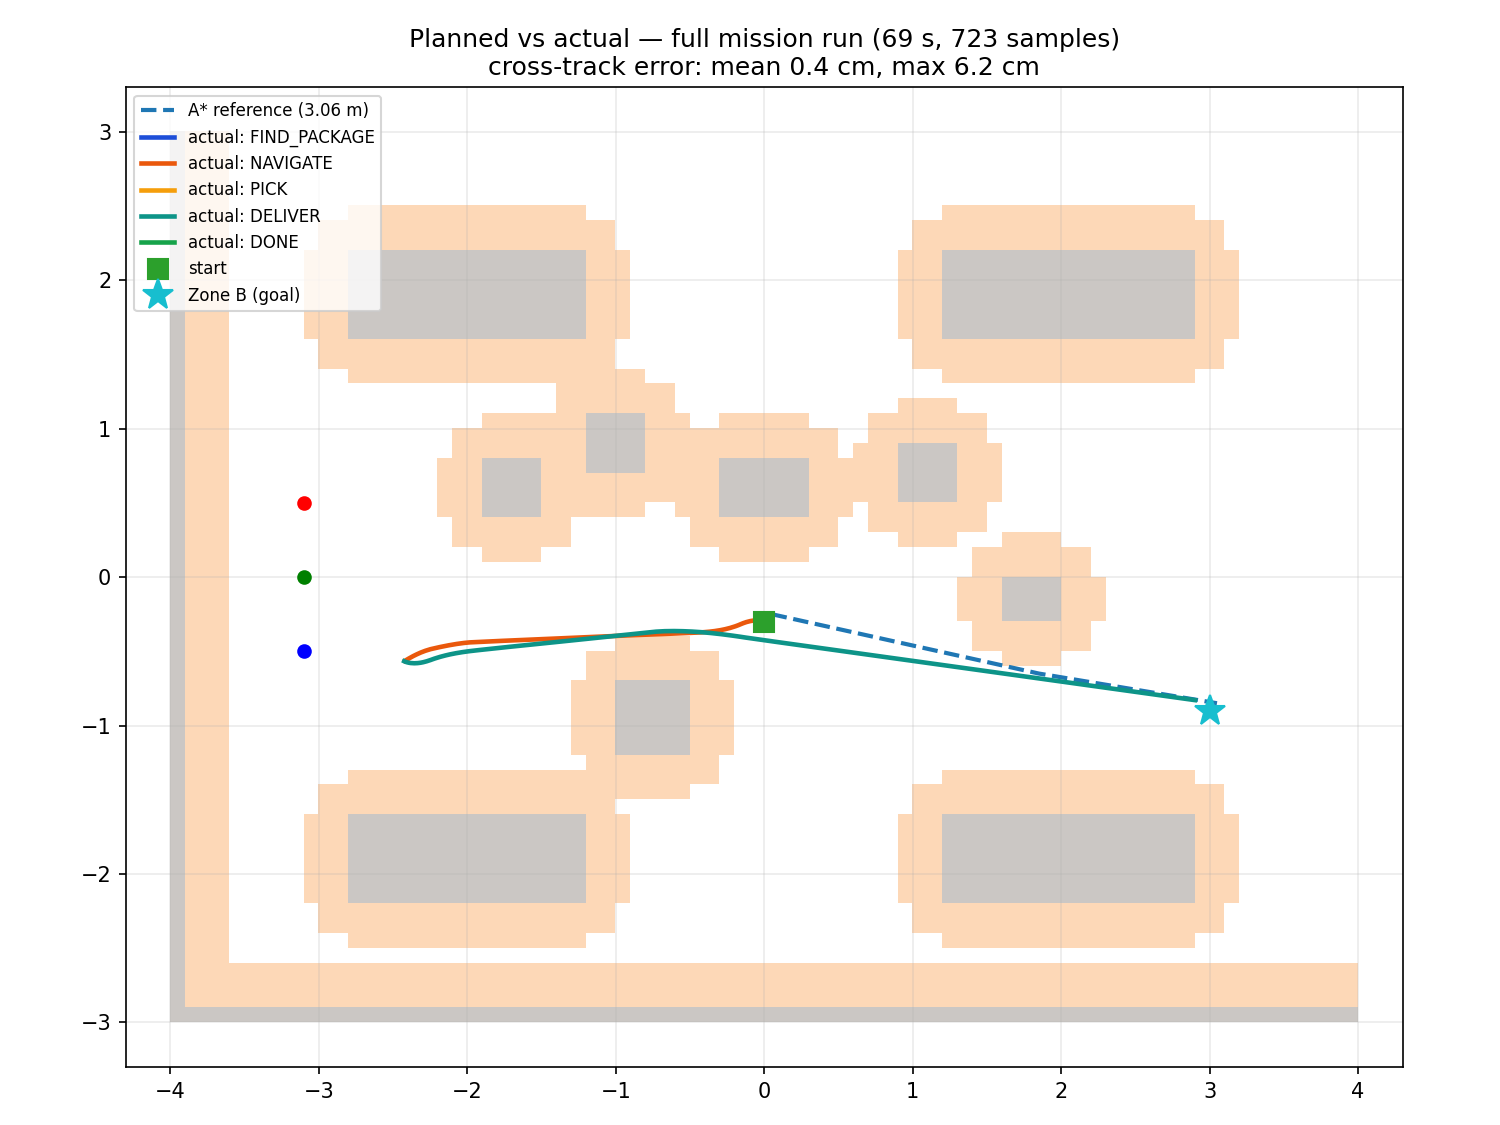
\includegraphics[width=\columnwidth]{figures/fig9_path.png}
\caption{A* reference (dashed) and the driven path coloured by FSM state, from a Webots mission log (69 s, 723 samples). Orange cells are the 0.25 m inflation around obstacles.}
\end{figure}
\subsection{Localisation: Why the EKF}
The offline ablation (Fig. 10) compares three navigation poses on the same mission. Odometry alone drifts to 22 cm RMSE. Raw GPS is noisy and failed the mission at docking (it needs centimetre accuracy). The EKF stays at 1.1 cm and only reaches 1.7 cm through a 10 s GPS outage, because odometry and IMU carry it through. When the robot is displaced mid-route, relocalisation cuts the error from 15.9 cm to 5.2 cm RMSE and the mission time from 93.6 s to 73.4 s.

\begin{figure*}[!t]
\centering
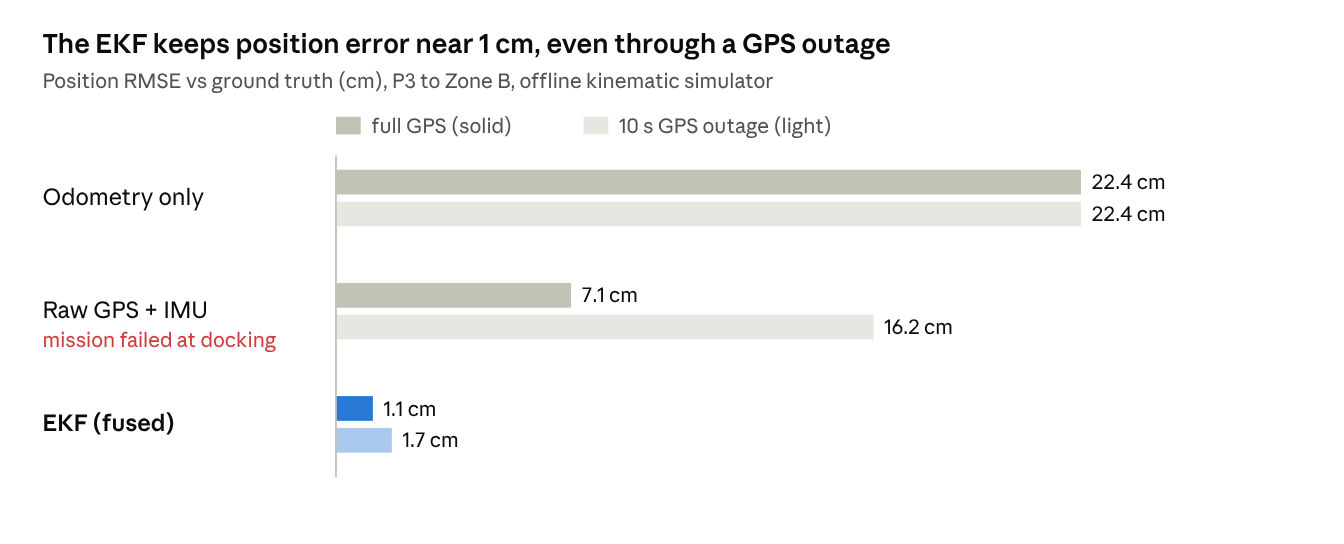
\includegraphics[width=0.9\textwidth]{figures/fig10_ablation.png}
\caption{Offline ablation of the navigation pose source (\texttt{tools/run\_\allowbreak{}experiments.py}).}
\end{figure*}
\subsection{Speed Governor and Dynamic Replanning}
Offline, the governor made missions 3--4 \% faster than a fixed 0.30 m/s (72.8 s vs 76.2 s for P3 to B) while keeping the same clearance and zero contacts. With a box appearing on the route, continuous replanning detoured early (PATH\_BLOCKED) and finished in 73.5 s with 0.20 m clearance; the legacy safety-stop approach got within 0.10 m and took 82.2 s. A cart crossing at 0.4 m/s still caused contacts in both variants in that model, which is what led to the give-way behaviour of the movers in Webots.

\subsection{Problems Found and Fixed}
Testing exposed real bugs; each was traced to a root cause before it was fixed (Table V).

\begin{table*}[!t]
\caption{Problems found during testing, root causes and fixes}
\centering
\footnotesize
\renewcommand{\arraystretch}{1.2}
\begin{tabular}{p{0.27\linewidth}p{0.38\linewidth}p{0.27\linewidth}}
\hline
\textbf{Symptom} & \textbf{Root cause} & \textbf{Fix} \\ \hline
Webots aborted with 0x40000015 after a few minutes; NumPy MemoryError & Webots R2025a leaks memory on every \texttt{Display.setFont()} call; the dashboard called it 3 times per refresh, so Webots grew $\sim$60--80 MB/s to $\sim$10 GB & set the font once and paste the static map as one image; memory now plateaus at 600--735 MB \\
27 rear-bumper hits, $-$0.17 m clearance, 21$^\circ$ heading RMSE in one run & a velocity-forced 0.75 m/s sphere rammed the waiting robot and a crate on every pass & slower lane clear of the crate, kinematic movers that give way, decoy robot \\
Moving obstacle froze mid-aisle; robot deadlocked behind it & the physics engine put the commanded body to sleep & kinematic movers (pose written every step) \\
DOCK\_PICK failed: parcel face not found by LiDAR & the arm post blinds $\pm6^\circ$ behind the LiDAR; parcel range fell back to a bounding box 0.3 m short & turn the parcel out of the rear blind sector before trusting range \\
Robot froze silently & stuck detection used the governed command, which was 0 while held & stuck check uses the pre-governor command \\
Camera health flapped to FROZEN & identical frames while standing still counted as frozen & count only while the base moves \\
\hline
\end{tabular}
\end{table*}
One more bug surfaced in the GUI run above. When the operator asked for P1 a second time, after it was already on the rack, the camera saw P1 on the rack. That estimate was more than 1.5 m from the pickup position, so the sanity check snapped it back to the empty pickup spot, and docking failed with PARCEL\_FACE\_NOT\_FOUND\_BY\_LIDAR, ending the session in ERROR. The robot now checks its own rack record first and rejects the task (``P1 is already on rack slot RA-L1-B1''), returning to the task prompt.

\subsection{Discussion}
The EKF is the component that made everything else possible: docking needs centimetre poses, and only the fused estimate delivered them, even through a simulated GPS outage. Making the speed limit a function of clearance let us raise cruise speed from 0.30 to 0.70 m/s without losing margin. The biggest lessons came from the simulator itself: two of the worst failures (the memory leak and the frozen obstacle) were Webots behaviours, not algorithm bugs, and were only found because every run wrote logs we could read afterwards. Results are still limited: the Webots numbers come from a few runs per configuration, the 10-run campaign predates the arm, and the Webots GPS is noise-free, which flatters localisation.

\section{Conclusion}
IntelliBot meets the project's objectives in simulation: it finds, picks, carries and places a parcel autonomously, through moving traffic, with centimetre-level accuracy and no contacts.

\begin{itemize}
\item \textbf{Closed loop, not scripted.} Every route comes from A* on the robot's own map, every parcel position from its cameras and LiDAR, and the parcel is physically held by the gripper.
\item \textbf{Fused localisation.} The EKF kept position error at 5--6 mm in Webots and rode through a 10 s GPS outage offline, where it was 20 times more accurate than odometry alone.
\item \textbf{Safe speed.} The clearance-based governor let cruise speed rise from 0.30 to 0.70 m/s with zero contacts in the reported runs.
\item \textbf{Engineering discipline.} One configuration generates both the world and the map, 312 tests run without the simulator, and every run leaves logs that let us find root causes, including a simulator memory leak.
\end{itemize}
The main limits are honest ones: few Webots runs per configuration, a noise-free simulated GPS, and a single robot.

\section{Future Work}
\begin{enumerate}
\item \textbf{Statistical evaluation.} Run each scenario (normal and ablations) at least 20 times in Webots and report success rates with confidence intervals.
\item \textbf{LiDAR map matching or SLAM.} Localise against the shelves themselves, so the robot no longer depends on GPS, which does not exist indoors in a real warehouse.
\item \textbf{Realistic GPS/indoor positioning noise.} Add bias, multipath and outages to the simulated GPS so the EKF is tested as it would be on hardware.
\item \textbf{Multi-robot fleet.} Turn the decoy robot into a real second IntelliBot and use the existing fleet manager and traffic reservations to share aisles.
\item \textbf{Learned perception.} Replace colour thresholds with a small object detector trained on simulator frames, so parcels need not have saturated colours.
\item \textbf{Retrieve missions.} Pick from shelves back to a zone; this needs a higher-reach arm or a lift for level 3.
\item \textbf{Hardware.} Port the plain-Python core to ROS 2 and a real differential-drive base with a low-cost arm.
\end{enumerate}
\begin{thebibliography}{00}
\bibitem{r1} Cyberbotics Ltd., \textit{Webots: Open-Source Robot Simulator}, version R2025a. [Online]. Available: \url{https://cyberbotics.com/doc/reference/index}
\bibitem{r2} S. Thrun, W. Burgard, and D. Fox, \textit{Probabilistic Robotics}. Cambridge, MA, USA: MIT Press, 2005.
\bibitem{r3} P. E. Hart, N. J. Nilsson, and B. Raphael, ``A formal basis for the heuristic determination of minimum cost paths,'' \textit{IEEE Trans. Syst. Sci. Cybern.}, vol. 4, no. 2, pp. 100--107, 1968.
\bibitem{r4} R. Siegwart, I. R. Nourbakhsh, and D. Scaramuzza, \textit{Introduction to Autonomous Mobile Robots}, 2nd ed. Cambridge, MA, USA: MIT Press, 2011.
\bibitem{r5} J. J. Craig, \textit{Introduction to Robotics: Mechanics and Control}, 4th ed. London, U.K.: Pearson, 2017.
\bibitem{r6} D. Fox, W. Burgard, and S. Thrun, ``The dynamic window approach to collision avoidance,'' \textit{IEEE Robot. Autom. Mag.}, vol. 4, no. 1, pp. 23--33, 1997.
\bibitem{r7} Y. Bar-Shalom, X. R. Li, and T. Kirubarajan, \textit{Estimation with Applications to Tracking and Navigation}. New York, NY, USA: Wiley, 2001.
\bibitem{r8} G. Bradski, ``The OpenCV library,'' \textit{Dr. Dobb's J. Softw. Tools}, 2000.
\bibitem{r9} C. R. Harris \textit{et al.}, ``Array programming with NumPy,'' \textit{Nature}, vol. 585, pp. 357--362, 2020.
\bibitem{r10} K. J. \AA{}str\"om and R. M. Murray, \textit{Feedback Systems: An Introduction for Scientists and Engineers}, 2nd ed. Princeton, NJ, USA: Princeton Univ. Press, 2021.
\end{thebibliography}
\end{document}
